% This must be in the first 5 lines to tell arXiv to use pdfLaTeX, which is strongly recommended.
% \pdfoutput=1
% In particular, the hyperref package requires pdfLaTeX in order to break URLs across lines.

\documentclass[11pt]{article}

% Remove the "review" option to generate the final version.
% \usepackage[review]{ACL2023}
\usepackage[]{ACL2023}

% Standard package includes
\usepackage{times}
\usepackage{latexsym}

% For proper rendering and hyphenation of words containing Latin characters (including in bib files)
\usepackage[T1]{fontenc}
% For Vietnamese characters
% \usepackage[T5]{fontenc}
% See https://www.latex-project.org/help/documentation/encguide.pdf for other character sets

% This assumes your files are encoded as UTF8
\usepackage[utf8]{inputenc}

% This is not strictly necessary, and may be commented out.
% However, it will improve the layout of the manuscript,
% and will typically save some space.
\usepackage{microtype}

% This is also not strictly necessary, and may be commented out.
% However, it will improve the aesthetics of text in
% the typewriter font.
\usepackage{inconsolata}

\usepackage{booktabs}
\usepackage{tikz}
\usepackage[autostyle, english=american]{csquotes}
\MakeOuterQuote{"}
\usepackage{subcaption}

\usepackage{amsmath}
\DeclareMathOperator{\PPL}{PPL}
\DeclareMathOperator{\PPPL}{PPPL}

% If the title and author information does not fit in the area allocated, uncomment the following
%
%\setlength\titlebox{<dim>}
%
% and set <dim> to something 5cm or larger.

\title{Perplexity as a Measure for Temporal Common Sense in Pre-Trained Language Models}

% Author information can be set in various styles:
% For several authors from the same institution:
% \author{Author 1 \and ... \and Author n \\
%         Address line \\ ... \\ Address line}
% if the names do not fit well on one line use
%         Author 1 \\ {\bf Author 2} \\ ... \\ {\bf Author n} \\
% For authors from different institutions:
% \author{Author 1 \\ Address line \\  ... \\ Address line
%         \And  ... \And
%         Author n \\ Address line \\ ... \\ Address line}
% To start a seperate ``row'' of authors use \AND, as in
% \author{Author 1 \\ Address line \\  ... \\ Address line
%         \AND
%         Author 2 \\ Address line \\ ... \\ Address line \And
%         Author 3 \\ Address line \\ ... \\ Address line}

% \author{First Author \\
%   Affiliation / Address line 1 \\
%   Affiliation / Address line 2 \\
%   Affiliation / Address line 3 \\
%   \texttt{email@domain} \\\And
%   Second Author \\
%   Affiliation / Address line 1 \\
%   Affiliation / Address line 2 \\
%   Affiliation / Address line 3 \\
%   \texttt{email@domain} \\}
 
\author{Tai Mai \\
  \texttt{mai@cl.uni-heidelberg.de} \\
  \\}

\begin{document}
\maketitle
\begin{abstract}
  Pre-trained language models are thought to learn both linguistic capabilities, as well as factual knowledge and common sense during their pre-training. To measure and interact with the unadulterated intuition obtained during pre-training, the pre-trained language model has to be used as is, without any further training such as fine-tuning. As a case study, this project attempts to capture the temporal common sense of pre-trained language models such as GPT-2, RoBERTa-base and Llama-3.1, using perplexity as an indicator and Allen's interval calculus as the annotation scheme for representing temporal relations. Two hypotheses are posed which relate back to the assumption that sentences reflecting common sense should be associated with a lower perplexity than sentences that do not. A dataset is constructed automatically and curated manually. The results of experiments conducted in this project did not support the hypotheses, indicating a possible fault in the data design or experimental setup.
\end{abstract}

\section{Introduction}

Language models nowadays see an ever increasing amount of data during their pre-training. For example, GPT-2 \citep{gpt2} was trained on 40 GB of text scraped from the web. RoBERTa \citep{roberta} was trained on over 160 GB of text, comprised of books, Wikipedia and news articles, as well as text scraped from the web. Llama-3.1 \citep{llama3} is a very recent model that was trained on over 15 trillion tokens of publicly available online data. While these figures are not directly comparable, they speak to the vast amounts data that are used to pre-train a language model. Language models are typically pre-trained in an unsupervised manner. For example, causal language models, such as GPT-2 \citep{gpt2} and Llama-3.1, \citep{llama3} generate text by predicting tokens one by one, each conditioned on the preceding tokens. Their objective is to correctly model their training data by maximizing the likelihood of token sequences that are present in the training data. On the other hand, masked language models, such as RoBERTa \citep{roberta}, are trained on another unsupervised task known as masked language modeling. In contrast to causal language modeling, masked language modeling is the process of randomly masking tokens in a training sentence and tasking the language model with reconstructing the original sentence based on the context surrounding the masked token. Pre-training a language model is designed to enable it to form an intuition for the language such that the resulting foundation model's intuition can be built upon in different downstream tasks, such as classification. This process of specializing a language model for a specific downstream task is called fine-tuning and often entails adding and training a few additional neural layers --- commonly called a task head --- to the pre-trained model to make it compatible with the desired downstream task. Besides obtaining an intuition for the language, pre-trained language models have also been shown to be able to form a semblance of factual common sense through pre-training \citep{evaluating}. However, testing a pre-trained language model for common sense in, say, temporal relations can be tricky. For example, employing a language model to classify the relation between two events in time is, in its most straight-forward form, a classification task that would most commonly require fine-tuning a classification head on top of the pre-trained model. Querying a model after fine-tuning, however, makes it impossible to say whether its understanding of time was obtained during pre-training or as a result of fine-tuning. To isolate the effects of pre-training alone, this kind of evaluation has to be done on the foundation model directly, without any further training.

This project attempts an approach to investigate the amount of temporal common sense that different pre-trained foundation language models obtain through pre-training. In lieu of fine-tuning the model for a classification task, the foundation model's perplexity metric is chosen as a proxy for how natural it judges a particular sentence. The results show that this implementation of perplexity is perhaps not a good measure to correlate with temporal common sense.



\section{Methods} % (fold)
\label{sec:Methods}

\subsection{Perplexity metrics}
\label{sec:ppl}
Perplexity in language models can be interpreted as a measure of how likely a language model thinks a token sequence is. The higher the perplexity metric is for a particular sequence, the more "surprised" the language model is to see that sequence. Perplexity is most commonly used for causal language modeling (CLM) and is defined as follows\footnote{\url{https://huggingface.co/docs/transformers/en/perplexity}},
\begin{equation}
  \PPL(X) = \exp \left\{ - \frac{1}{t} \sum^t_i \log p_\text{CLM} (x_i | x_{<i}) \right\},
  \label{eq:ppl}
\end{equation}
where $X$ denotes the token sequence of tokens $x$, $t$ is the number of tokens in the sequence, and $p(x_i | x_{<i})$ represents the probability of token $x_i$ at position $i$, given all the previous tokens $x_{<i}$. Therefore, this definition of perplexity is very specific to causal language modeling and cannot be directly applied to masked language modeling.

To obtain an analogous metric for masked language modeling (MLM), \citet{pppl} propose the following pseudo-perplexity metric.
\begin{equation}
  \PPPL(X) := \exp \left\{ - \frac{1}{t} \sum^t_i \log p_\text{MLM} (x_i | X_{\backslash x_i}) \right\}
  \label{eq:pppl}
\end{equation}
The only difference to Equation~\ref{eq:ppl} is in the context on which the token $x_i$ is conditioned. In causal language modeling, the choice of token $x_i$ at position $i$ is conditioned on all tokens to the left of position $i$. Future tokens cannot be taken into account in causal language modeling, therefore the context is unilateral. In masked language modeling, however, tokens in the sequence are chosen and masked at random. To reconstruct a masked token $x_i$, masked language models are provided with all other unmasked tokens in the sequence, both before and after position $i$. Therefore, the context in masked language modeling is bilateral.

These metrics are chosen to gauge how natural a language model thinks a sequence is, specifically in the case of temporal relations described in the following section.

\subsection{Allen's Interval Calculus}
\label{sec:allen}
\citet{allen} proposes a system of relating two events, $e_1$ and $e_2$, to each other in time via a set of basic temporal relations. This set can be boiled down to the following seven relations.

\begin{itemize}
  \item \textit{before}$(e_1, e_2)$: $e_1$ starts and ends before $e_2$ starts
  \item \textit{meets}$(e_1, e_2)$: $e_1$ starts before $e_2$ and $e_2$ starts when $e_1$ ends
  \item \textit{overlaps}$(e_1, e_2)$: $e_1$ starts before $e_2$ and $e_1$ ends between the start and end of $e_2$
  \item \textit{starts}$(e_1, e_2)$: $e_1$ starts at the same time as $e_2$ and $e_1$ ends before $e_2$
  \item \textit{during}$(e_1, e_2)$: $e_1$ starts after $e_2$ and $e_1$ ends before $e_2$
  \item \textit{finishes}$(e_1, e_2)$: $e_1$ starts after $e_2$ and $e_1$ ends at the same time as $e_2$
  \item \textit{equals}$(e_1, e_2)$: $e_1$ starts and ends at the same time as $e_2$
\end{itemize}

The complete set proposed by \citet{allen} also contains inverses of the previous relations. However, these inverses can also be modeled by the seven relations above by simply swapping the positions of the events as arguments to the relations, i.e.~\textit{after}$(e_1, e_2)$ is equivalent to \textit{before}$(e_2, e_1)$. Therefore, this project will only consider the seven relations mentioned above. These relations can then also be verbalized into natural language. For example, one possible template verbalization of the relation \textit{before} could be "$e_1$ \textit{happens before} $e_2$." An event tuple such as $\langle \text{birth}, \text{death} \rangle$ can then be connected and verbalized as \textit{"Birth happens before death."} The objective of this project is to investigate how well the perplexity values of these verbalizations correlate with temporal common sense. Specifically, the first hypothesis investigated in this project is that a verbalization that reflects temporal common sense, such as \textit{"Birth happens before death,"} should receive a lower perplexity score than one that does not reflect temporal common sense, such as \textit{"Birth happens during death."}

\subsection{Conceptual Neighborhood}

\begin{figure}
  \begin{center}
    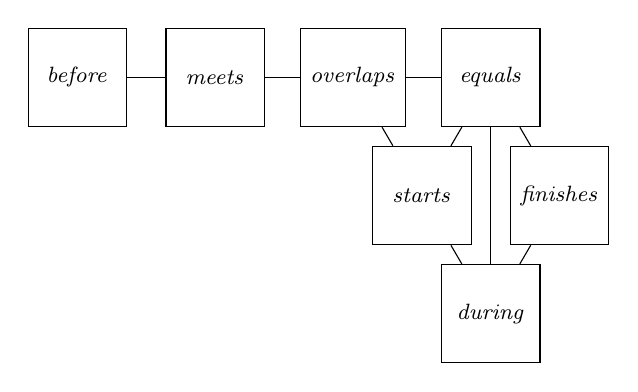
\begin{tikzpicture}[node distance=2cm, every node/.style={draw, minimum size=1.25cm, font=\footnotesize, text centered}]
      % Nodes
      \node (before) at (0, 0) {\textit{before}};
      \node (meets) at (1.75, 0) {\textit{meets}};
      \node (overlaps) at (3.5, 0) {\textit{overlaps}};
      \node (equals) at (5.25, 0) {\textit{equals}};
      \node (during) at (5.25, -3) {\textit{during}};
      \node (starts) at (4.375, -1.5) {\textit{starts}};
      \node (finishes) at (6.125, -1.5) {\textit{finishes}};

      % Edges
      \draw (before) -- (meets);
      \draw (meets) -- (overlaps);
      \draw (overlaps) -- (equals);
      \draw (overlaps) -- (starts);
      \draw (equals) -- (starts);
      \draw (equals) -- (during);
      \draw (equals) -- (finishes);
      \draw (starts) -- (during);
      \draw (finishes) -- (during);
    \end{tikzpicture}
  \end{center}
  \caption{Conceptual neighborhood according to \citet{freksa}, excluding the inverse relations.}
  \label{fig:conceptual_neighborhood}
\end{figure}


\citet{freksa} arranges the relations proposed by \citet{allen} in an undirected graph structure to encode how closely the relations are related to each other. Figure~\ref{fig:conceptual_neighborhood} shows this graph after excluding the inverse relations. With this graph structure in mind, this project attempts to investigate whether the perplexity scores correlate with the conceptual distance in graph hops. As an example, the relations \textit{before} and \textit{during} are separated by four node hops in the conceptual neighborhood graph. As mentioned in Section~\ref{sec:allen}, we hypothesize that an atypical verbalization, such as \textit{"Birth happens during death,"} should receive a higher perplexity score than a common sense verbalization, such as \textit{"Birth happens before death."} Therefore, the second hypothesis investigated in this project is that this change in perplexity should correlate with the degrees of separation between the two relations when plugging an event tuple from one relation into a verbalization of another relation.

\section{Data}
\label{sec:data}
To test these two hypotheses, a dataset containing examples of Allen's interval calculus relations is needed. Since such a dataset does not exist to the best our knowledge, a simple dataset has been constructed by utilizing Claude-3.5 Sonnet\footnote{\url{https://www.anthropic.com/news/claude-3-5-sonnet}} and then curated by hand. For each of the $7$ temporal relations, a set of $20$ event tuples are gathered as examples of the temporal relation in question. For the relation \textit{before}, one of the examples collected is the tuple $\langle \text{birth}, \text{death}\rangle$.
Furthermore, for each of the relations, a set of $10$ possible template verbalizations is collected, with \texttt{\{event1\}} and \texttt{\{event2\}} as placeholders for respective temporal events, for example \textit{"\texttt{\{event1\}} happens before \texttt{\{event2\}}."}
When placing every event tuple into every template verbalization of every relation, this yields a total dataset size of $20 \cdot 10 \cdot 7 = 1400$ verbalized examples.

Before Claude-3.5 Sonnet was released, GPT-3.5 and GPT-4o\footnote{\url{https://chatgpt.com}} were also considered for the task of generating the dataset. However, upon manual inspection of the generated data, these models did not prove to be able to come up with (enough) correct and/or diverse examples and were subsequently dropped in favor of Claude-3.5 Sonnet, which required a lot less manual intervention. The prompting steps used to generate this dataset can be seen in Appendix~\ref{sec:prompts}. The dataset and code can be accessed publicly online\footnote{\url{https://github.com/Tai-Mai/temporal-common-sense/blob/main/data/claude_examples.json}}.

\section{Evaluation} % (fold)
\label{sec:Evaluation}

\subsection{Confusion Matrices}

\subsubsection{Relation Prediction}

To relate back to the classification task, the perplexity values can theoretically be used to predict the correct relation. As explained in Section~\ref{sec:data}, a set of $20$ event tuples are collected as examples for every relation. One such example for the relation \textit{before} is the event tuple $\langle \text{birth}, \text{death} \rangle$. This event tuple is then plugged into all $10$ template verbalizations of each of the $7$ relations, resulting in verbalizations such as \textit{"Birth happens during death."} The perplexity values are then aggregated as averages for each verbalized relation across all its $10$ template verbalizations. 
The relation whose template verbalizations achieve the lowest perplexity scores on average is then chosen as the predicted relation. Under the first hypothesis, verbalizing with the correct relation's templates should receive lower perplexity scores than the other, more atypical relations. This can be represented as a confusion matrix that contains a tally of how often a relation (in the columns) was predicted for an event tuple coming from its true relation (in the rows). Figure~\ref{fig:confusion_matrix_counts} shows the resulting confusion matrices.

\begin{figure*}
  \centering
    \begin{subfigure}[b]{0.45\textwidth}
      \centering
      \includegraphics[width=0.95\columnwidth, height=0.75\textheight, keepaspectratio, valign=c]{../plots/gpt2_confusion_matrix_counts.pdf}
      \caption{GPT-2}
    \end{subfigure}
    \begin{subfigure}[b]{0.45\textwidth}
      \centering
      \includegraphics[width=0.95\columnwidth, height=0.75\textheight, keepaspectratio, valign=c]{../plots/gpt2_confusion_matrix_counts_normalized.pdf}
      \caption{GPT-2 (normalized)}
    \end{subfigure}

    \vspace{1em}

    \begin{subfigure}[b]{0.45\textwidth}
      \centering
      \includegraphics[width=0.95\columnwidth, height=0.75\textheight, keepaspectratio, valign=c]{../plots/roberta-base_confusion_matrix_counts.pdf}
      \caption{RoBERTa-base}
    \end{subfigure}
    \begin{subfigure}[b]{0.45\textwidth}
      \centering
      \includegraphics[width=0.95\columnwidth, height=0.75\textheight, keepaspectratio, valign=c]{../plots/roberta-base_confusion_matrix_counts_normalized.pdf}
      \caption{RoBERTa-base (normalized)}
    \end{subfigure}

    \vspace{1em}

    \begin{subfigure}[b]{0.45\textwidth}
      \centering
      \includegraphics[width=0.95\columnwidth, height=0.75\textheight, keepaspectratio, valign=c]{../plots/meta-llama-3-1-8b_confusion_matrix_counts.pdf}
      \caption{Llama-3.1}
    \end{subfigure}
    \begin{subfigure}[b]{0.45\textwidth}
      \centering
      \includegraphics[width=0.95\columnwidth, height=0.75\textheight, keepaspectratio, valign=c]{../plots/meta-llama-3-1-8b_confusion_matrix_counts_normalized.pdf}
      \caption{Llama-3.1 (normalized)}
    \end{subfigure}
  \caption{Counts of predicted relations (columns), given the event tuples from the true relation (rows).}
  \label{fig:confusion_matrix_counts}
\end{figure*}

Assuming the first hypothesis investigated in this project, the perplexity values should be lowest on the matrices' diagonals and higher for off-diagonal cells. Therefore, one might expect the diagonals in the confusion matrices to contain the highest prediction counts. However, this does not prove to be the case. Instead, there seems to emerge a similar pattern among all three models where the columns \textit{overlaps} and \textit{equals} tend to contain the highest counts. This seems to indicate that the perplexity values are highly dependent on the template verbalizations. If a template verbalization already contains an unlikely sequence of tokens before plugging in an actual event tuple, it could dominate the perplexity value and obscure any effect that the event tuple has.

As an attempt to mitigate this effect, a strategy to normalize the perplexity values was devised. Instead of choosing the raw perplexity values for the predictions, as has been the case until now, the perplexity values are normalized by using reference verbalizations. A reference verbalization is constructed by substituting the placeholders \texttt{\{event1\}} and \texttt{\{event2\}} in the template with "an event" and "another event," respectively. In the case of the relation \textit{before}, one such reference verbalization would be \textit{"An event happens before another event"}.
\begin{equation}
  \frac{\PPL\left(\textit{before}(\text{"birth"}, \text{"death"})\right)}{\PPL\left(\textit{before}(\text{"an event"}, \text{"another event"})\right)}.
\end{equation}
This is done to cancel out the effects of the verbalization by itself and distill the effect of the \emph{interaction} between the event tuples and the verbalizations in the ratio. In the case of masked language models, the perplexity metric $\PPL(\cdot)$ can be substituted with the pseudo-perplexity $\PPPL(\cdot)$. Choosing the lowest average perplexity ratio for the prediction yields the normalized confusion matrices in Figure~\ref{fig:confusion_matrix_counts}. Unfortunately, this strategy does not seem to have the desired effect, as an even more concentrated column pattern seems to emerge.

\subsubsection{Perplexities}
\label{sec:perplexities}
Instead of visualizing the prediction counts, we further opt to visualize the perplexity values themselves.
This results in new confusion matrices with the original, true relation in the rows and the verbalized relation in the columns, as can be seen in Figure~\ref{fig:confusion_matrix_values}. 
\begin{figure*}
  \centering
    \begin{subfigure}[b]{0.95\textwidth}
      \centering
      \includegraphics[width=0.95\columnwidth, height=0.3\textheight, keepaspectratio, valign=c]{../plots/gpt2_confusion_matrix_values.pdf}
      \caption{GPT-2}
    \end{subfigure}

    \vspace{1em}

    \begin{subfigure}[b]{0.95\textwidth}
      \centering
      \includegraphics[width=0.95\columnwidth, height=0.3\textheight, keepaspectratio, valign=c]{../plots/roberta-base_confusion_matrix_values.pdf}
      \caption{RoBERTa-base}
    \end{subfigure}

    \vspace{1em}

    \begin{subfigure}[b]{0.95\textwidth}
      \centering
      \includegraphics[width=0.95\columnwidth, height=0.3\textheight, keepaspectratio, valign=c]{../plots/meta-llama-3-1-8b_confusion_matrix_values.pdf}
      \caption{Llama-3.1}
    \end{subfigure}
  \caption{Average perplexity values when plugging event tuples from the true relation (rows) into verbalizations of all other relations (columns). For the masked language model RoBERTa-base, the pseudo-perplexity is shown instead.}
  \label{fig:confusion_matrix_values}
\end{figure*}

Consistent with the previous confusion matrices, verbalizing event tuples with the relation \textit{overlaps} and \textit{equals} tends to result in relatively low perplexity values compared to other relations. This manifests as dark \textit{overlaps} and \textit{finishes} columns in the heat map. Meanwhile, the \textit{finishes} column contains the highest perplexity value in all three models. 

Once again, the strategy to normalize the perplexity values was employed and the resulting perplexity value ratios are displayed in the confusion matrices.
This time, this strategy seems to be successful in removing the column pattern observed before, as can be seen in Figure~\ref{fig:confusion_matrix_values_normalized}. Numerically, one can observe that most of these ratios are greater than $1$, indicating that the specific verbalizations with instantiated events obtain higher perplexity values than the generic reference verbalizations. Only in the case of Llama-3.1, the \textit{equals} row consistently contains ratios smaller than $1$.
In fact, while the column pattern has been mitigated, the \textit{equals} row brings to attention another pattern that emerges in the rows of the confusion matrices. In all three models, the \textit{equals} row contains the lowest perplexity ratios in all columns. This suggests that the event tuples from the relation \textit{equals} are associated with lower perplexity scores, no matter which relation they are verbalized with. For both causal language models, GPT-2 and Llama-3.1, a similar pattern can be observed in the \textit{before} and \textit{overlaps} rows which tend to be brighter than the other rows, indicating that the event tuples from these relations tend to be associated with higher perplexity values, regardless of the relation they are verbalized with.

\begin{figure*}
  \centering
    \begin{subfigure}[b]{0.95\textwidth}
      \centering
      \includegraphics[width=0.95\columnwidth, height=0.3\textheight, keepaspectratio, valign=c]{../plots/gpt2_confusion_matrix_values_normalized.pdf}
      \caption{GPT-2}
    \end{subfigure}

    \vspace{1em}

    \begin{subfigure}[b]{0.95\textwidth}
      \centering
      \includegraphics[width=0.95\columnwidth, height=0.3\textheight, keepaspectratio, valign=c]{../plots/roberta-base_confusion_matrix_values_normalized.pdf}
      \caption{RoBERTa-base}
    \end{subfigure}

    \vspace{1em}

    \begin{subfigure}[b]{0.95\textwidth}
      \centering
      \includegraphics[width=0.95\columnwidth, height=0.3\textheight, keepaspectratio, valign=c]{../plots/meta-llama-3-1-8b_confusion_matrix_values_normalized.pdf}
      \caption{Llama-3.1}
    \end{subfigure}
  \caption{Average perplexity ratios \textit{after normalizing} the perplexity values. Perplexity values are normalized by dividing by the perplexity values of reference verbalizations. True relation in the rows, verbalized relation in the columns. For the masked language model RoBERTa-base, the pseudo-perplexity ratio is shown instead.}
  \label{fig:confusion_matrix_values_normalized}
\end{figure*}

\subsection{Correlation Analysis}
As discussed in Section~\ref{sec:perplexities}, the hypothesized diagonal pattern did not seem to be discernible. To confirm this observation quantitatively, we evaluate the second hypothesis of this project. Under the second hypothesis, when verbalizing an event tuple $\langle e_1, e_2 \rangle$ using another relation than its original relation $\textit{rel}_\text{og}$, the perplexity values $\PPL(\cdot)$ should scale according to the conceptual distance $d_\text{hops}(\textit{rel}, \textit{rel}_\text{og})$ between the original relation and the confused relation, measured in graph hops in Freksa's conceptual neighborhood graph (Figure~\ref{fig:conceptual_neighborhood}). For example, the hypothesis assumes for the event tuple $\langle \text{birth}, \text{death} \rangle$ that
\begin{equation}
  \PPL(\textit{meets}(\text{birth}, \text{death})) < \PPL(\textit{finishes}(\text{birth}, \text{death})),
\end{equation}
because \textit{meets} is conceptually closer to the tuple's original relation \textit{before} ($d_\text{hops}(\textit{meets}, \textit{before}) = 1$) than \textit{finishes} is ($d_\text{hops}(\textit{finishes}, \textit{before}) = 4$).
This means that an event tuple $\langle e_1, e_2 \rangle$ should receive higher absolute perplexity scores when verbalized using wrong relations $\textit{rel}(e_1, e_2)$ that are more conceptually distant from the tuple's original relation $\textit{rel}_\text{og}(e_1, e_2)$, compared to relations that are conceptually closer to $\textit{rel}_\text{og}$. Formally, we investigate the following correlation for all relations \textit{rel} and all event tuples $\langle e_1, e_2\rangle$:
\begin{equation}
  \text{Cor}\left(\PPL(\textit{rel}(e_1, e_2)), d_\text{hops}(\textit{rel}, \textit{rel}_\text{og}) \right)
\end{equation}

\begin{table*}
  \centering
  \begin{tabular}{l c c c}
    \toprule
    Model & $r$ & $\rho$ & $\tau$ \\
    \midrule
    % \arrayrulecolor{black! 30}\midrule  % needs \usepackage[table]{xcolor}
    GPT-2 & $0.0537$ & $0.0654$ & $0.0477$ \\
    GPT-2 (normalized) & $0.0407$ & $0.0608$ & $0.0444$ \\
    RoBERTa-base & $0.0266$ & $0.0906$ & $0.0661$ \\
    RoBERTa-base (normalized) & $0.0231$ & $0.0876$ & $0.0638$ \\
    Llama-3.1 8B & $0.0483$ & $0.1230$ & $0.0901$ \\
    Llama-3.1 8B (normalized) & $0.0571$ & $0.1212$ & $0.0884$ \\
    \bottomrule
    % \arrayrulecolor{black}\bottomrule % needs \usepackage[table]{xcolor}
  \end{tabular}
  \caption{Pearson's $r$, Spearman's $\rho$, and Kendall's $\tau$ correlation coefficients between \emph{absolute perplexity values} and graph hops.}
  \label{correlations_raw}
\end{table*}

\begin{table*}
  \centering
  \begin{tabular}{l c c c}
    \toprule
    Model & $r$ & $\rho$ & $\tau$ \\
    \midrule
    % \arrayrulecolor{black! 30}\midrule  % needs \usepackage[table]{xcolor}
    GPT-2 & $0.0319$ & $-0.0968$ & $-0.0698$ \\
    GPT-2 (normalized) & $0.0087$ & $-0.0419$ & $-0.0304$ \\
    RoBERTa-base & $0.0106$ & $-0.0484$ & $-0.0342$ \\
    RoBERTa-base (normalized) & $0.0094$ & $-0.0126$ & $-0.0087$ \\
    Llama-3.1 8B & $0.0242$ & $-0.0665$ & $-0.0469$ \\
    Llama-3.1 8B (normalized) & $0.0278$ & $-0.0224$ & $-0.0148$ \\
    \bottomrule
    % \arrayrulecolor{black}\bottomrule % needs \usepackage[table]{xcolor}
  \end{tabular}
  \caption{Pearson's $r$, Spearman's $\rho$, and Kendall's $\tau$ correlation coefficients between \emph{perplexity deltas} and graph hops.}
  \label{correlations_deltas}
\end{table*}

Table~\ref{correlations_raw} lists the correlation coefficients Pearson's $r$, Spearman's $\rho$, and Kendall's $\tau$. They confirm that there is no notable correlation between the absolute perplexity scores and conceptual distance in graph hops. One observation that could be made is that the Spearman's $\rho$ is slightly higher for Llama-3.1 compared to the weaker models GPT-2 and RoBERTa-base.

Instead of correlating the absolute perplexity values with the conceptual distance in graph hops, we try substituting it with the \emph{change} in perplexity $\Delta \PPL(\cdot)$, relative to the original relation's average perplexity.
\begin{equation}
  \text{Cor}\left(\Delta\PPL(\textit{rel}(e_1, e_2)), d_\text{hops}(\textit{rel}, \textit{rel}_\text{og}) \right)
\end{equation}
The rationale is the same as before: The change in perplexity should scale with the conceptual distance. Table~\ref{correlations_deltas} shows that Spearman's $\rho$ and Kendall's $\tau$ have now even switched to negative values while being of a similar magnitude as the previous values (near 0). 
This correlation analysis has therefore confirmed that this experimental setup does not exhibit any correlation between perplexity and conceptual distance.

\section{Discussion and Conclusion}

\begin{figure*}
  \centering
    \begin{subfigure}[b]{0.95\textwidth}
      \centering
      \includegraphics[width=0.95\columnwidth, height=0.3\textheight, keepaspectratio, valign=c]{../plots/gpt2_confusion_matrix_values_correlation.pdf}
      \caption{GPT-2}
    \end{subfigure}

    \vspace{1em}

    \begin{subfigure}[b]{0.95\textwidth}
      \centering
      \includegraphics[width=0.95\columnwidth, height=0.3\textheight, keepaspectratio, valign=c]{../plots/roberta-base_confusion_matrix_values_correlation.pdf}
      \caption{RoBERTa-base}
    \end{subfigure}

    \vspace{1em}

    \begin{subfigure}[b]{0.95\textwidth}
      \centering
      \includegraphics[width=0.95\columnwidth, height=0.3\textheight, keepaspectratio, valign=c]{../plots/meta-llama-3-1-8b_confusion_matrix_values_correlation.pdf}
      \caption{Llama-3.1}
    \end{subfigure}
  \caption{Absolute perplexity scores. For the masked language model RoBERTa-base, the pseudo-perplexity values are shown instead.}
  \label{fig:scatter}
\end{figure*}

This project aimed to investigate two hypotheses. The first hypothesis is that perplexity is higher for a temporal event tuple $\langle e_1, e_2 \rangle$ if it is verbalized with a wrong relation compared to when it is verbalized with a relation that reflects common sense. The second hypothesis is that the absolute perplexity values or relative perplexity changes are correlated with the conceptual distance between the confused relations, according to the conceptual neighborhood graph by \citet{freksa}. The experimental setup of this project was unable to prove these hypotheses. In fact, the results seem to contradict the two hypotheses, showing no notable correlation. However, while these results do not confirm the hypotheses, we cannot assume that they disprove them either. As can be seen in Figures~\ref{fig:confusion_matrix_values} and \ref{fig:confusion_matrix_values_normalized}, the standard deviations among the perplexities is often higher than the average itself. This indicates that the perplexity metric is very unstable and often yields very high outlier values that drive up the standard deviation. These outliers can be seen in the marginal box plots in Figure~\ref{fig:scatter}. We have to therefore assume that this experimental setup is invalid and does not adequately measure what it purports to measure. Two possible sources of error are faulty implementations of perplexity or pseudo-perplexity, or, somewhat more likely, a subpar design of the dataset. The dataset is intended to work in a way such that the event tuples can be plugged into all seven relations and still be more or less grammatically correct. The problem likely stems from the fact that, while grammatically correct, the resulting verbalizations are still very unnatural and do not reflect how humans would typically express them. For example, one of the template verbalizations for the relation \textit{before} is \textit{"\texttt{\{event1\}} starts and ends before \texttt{\{event2\}}"}. While this template accurately reflects the definition of the \textit{before} relation according to \citet{allen}, it is not how humans would typically phrase it in everyday speech. We suspect that this might be what could be driving up perplexity values for verbalizations, even if they conceptually agree with common sense. While the normalization strategy aimed to mitigate this issue, and seemed to be successful in Figure~\ref{fig:confusion_matrix_values_normalized}, it did not help in the prediction of the correct relation and also did not exhibit the hypothesized correlation. Further research has to be conducted to examine whether this could be indicating that Freksa's conceptual neighborhood graph does in fact not accurately reflect how language models intuit temporal relations.

To improve on this experimental setup, a more natural way to verbalize event tuples into relations could be devised. While the strategy employed in this project naively substitutes the placeholder events \texttt{\{event1\}} and \texttt{\{event2\}} with their respective examples, this can result in unnatural sentences. Instead, one might try to verbalize by hand or query a capable large language model to formulate it into a more natural sentence. Naturally, this has to be another language model than the ones that are being tested, therefore Llama-3.1 --- and arguably also Llama-2 --- are out of the question. Using APIs such as ChatGPT/GPT 4o, Gemini \citep{gemini}, or Claude 3.5 would require $20\cdot10\cdot7 = 1400$ additional paid API calls, which was out of the scope of this project. However, if budget permits, this might prove to be a viable option for future work to verbalize event tuples with relations more naturally.


\section{Related Works}
Previous research has corroborated the idea of language models, especially large language models, learning common sense during pre-training. \citet{task_planning} leverage the common sense of large language models for large-scale task planning. \citet{evaluating} evaluate the common sense in pre-trained language models similarly to this project, by scoring sentences from various benchmark datasets using the log-likelihoods of sentences, or the equivalent of pseudo-log-likelihoods for masked language models. \citet{better_scoring} propose an improved way of sequence scoring for masked language models, which changes which tokens in the sequence are masked. This improved strategy showed to be more robust for out-of-vocabulary words. However, this project chooses to keep the simpler pseudo-perplexity metric for ease of implementation. Like this project, \citet{overview}, too, concentrate on temporal common sense specifically and propose methods to enhance the language model's capabilities by augmentation in order for them not to default to linguistic heuristics. However, to the best of our knowledge, this project is the first to use Allen's interval calculus as an annotation scheme to capture temporal common sense.

% Entries for the entire Anthology, followed by custom entries
% \bibliography{anthology,custom}
\bibliography{references}
\bibliographystyle{acl_natbib}

\appendix
\onecolumn

\section{Appendix}
\subsection{Claude-3.5 Sonnet Prompting for the Dataset Generation}
\label{sec:prompts}
\begin{enumerate}
  \item What are the relations in James Allen's interval calculus?
    \begin{itemize}
      \item James Allen's Interval Calculus, introduced in 1983, defines 13 basic relations between time intervals. These relations describe all possible ways two time intervals can be related to each other. Here's a concise list of the 13 relations:
        \begin{enumerate}
          \item Before (precedes)
          \item Meets
          \item Overlaps
          \item Starts
          \item During
          \item Finishes
          \item Equals
          \item Finished-by
          \item Contains
          \item Started-by
          \item Overlapped-by
          \item Met-by
          \item After (follows)
        \end{enumerate}
These relations are mutually exclusive and exhaustive, meaning any two time intervals must be related by exactly one of these relations. Each relation also has an inverse (e.g., "before" is the inverse of "after"), which is why there are 13 relations instead of 7.
Would you like me to elaborate on any specific relation or provide examples of how these relations are used in temporal reasoning?
    \end{itemize}
  \item Give me the relations without the inverses
    \begin{itemize}
      \item Certainly. If we consider only the base relations without their inverses, we can reduce James Allen's Interval Calculus to 7 fundamental relations. Here they are:
        \begin{enumerate}
          \item Before
          \item Meets
          \item Overlaps
          \item Starts
          \item During
          \item Finishes
          \item Equals
        \end{enumerate}
These 7 relations form the core of Allen's Interval Calculus. The other 6 relations in the full set of 13 are inverses of these (except for "Equals," which is its own inverse).
Would you like me to explain how these relations are defined or provide examples of their use in temporal reasoning?
    \end{itemize}
  \item Please define each of these seven relations in Allen's Interval Calculus.
    \begin{itemize}
      \item Certainly. I'll define each of the seven base relations in Allen's Interval Calculus. Let's consider two time intervals, A and B:
        \begin{enumerate}
          \item Before (A before B):
            Interval A ends before interval B starts. There is a gap between A and B.
          \item Meets (A meets B):
            The end point of interval A is exactly the start point of interval B. There is no gap between them.
          \item Overlaps (A overlaps B):
            Interval A starts before B, and they overlap for some duration. A ends sometime after B starts but before B ends.
          \item Starts (A starts B):
            Both intervals start at the same point, but A ends before B ends.
          \item During (A during B):
            Interval A starts after B starts and ends before B ends. A is completely contained within B.
          \item Finishes (A finishes B):
            Both intervals end at the same point, but A starts after B starts.
          \item Equals (A equals B):
            Both intervals start and end at the same points. They are identical in duration and position.
        \end{enumerate}
        These definitions assume that intervals are non-zero in duration and have distinct start and end points. Each relation (except "Equals") has an inverse relation in the full set of 13 relations.
        Would you like me to provide visual representations or examples of these relations?
    \end{itemize}
  \item For each of these relations, give me 10 commonsense examples of temporal events or periods . They should always and universally be true. Don't use examples that are just "often" or "sometimes" the case. Make sure not to confuse "before" with "meets". Also, don't confuse "finishes" with "after". For "meets", don't mention the point in time where they meet. Format the examples in JSON like this:
    \{ "before": [ \{ "event1": "breakfast", "event2": "lunch", "example": "breakfast happens before lunch." \}, \{ "event1": ..., ... \}, ] ...\}
    \begin{itemize}
      \item I understand your request. I'll provide 10 commonsense examples for each of the seven relations in Allen's Interval Calculus, ensuring they are always and universally true. I'll format them in JSON as requested, being careful to distinguish between "before" and "meets", and between "finishes" and "after". Here's the JSON with the examples:
        [...]
  I've created a JSON structure with 10 examples for each of the seven relations in Allen's Interval Calculus. These examples are designed to be universally true and not just "often" or "sometimes" the case. I've been careful to distinguish between "before" and "meets", as well as between "finishes" and "after". For the "meets" relation, I've avoided mentioning the specific point in time where the events meet.
  Each relation has its own array of examples, and each example is structured with "event1", "event2", and an "example" sentence describing the relation between the events.
  Is there anything you'd like me to clarify or expand upon regarding these examples or Allen's Interval Calculus?
    \end{itemize}
  \item Please do the same thing again and create 10 new examples for each relation. Do not repeat the ones you've created so far. Take care that the "equals" relation needs to be about temporal periods only.
    \begin{itemize}
      \item Certainly, I'll create 10 new examples for each relation, ensuring they are distinct from the previous set and that the "equals" relation focuses solely on temporal periods. I'll maintain the same JSON structure and adhere to the guidelines you've provided.
        [...]
I've created a new set of 10 examples for each of the seven relations in Allen's Interval Calculus. These examples are distinct from the previous set and adhere to the guidelines you provided. For the "equals" relation, I've ensured that all examples focus solely on temporal periods.
Each relation is represented by an array of examples, with each example containing "event1", "event2", and an "example" sentence describing the relation between the events.
Is there anything you'd like me to clarify or expand upon regarding these new examples or Allen's Interval Calculus?
    \end{itemize}
  \item For each of the relations, generate me a list of possible verbalizations by using placeholders for the two events. Format it as JSON like this: \{ "before": [ "\{event1\} happens before \{event2\}" ... ], ... \}
    \begin{itemize}
      \item Certainly! I'll create a list of possible verbalizations for each of Allen's Interval Calculus relations, using placeholders for the two events. I'll format this as JSON as you've requested.
        [...]
        I've created a JSON structure with 10 possible verbalizations for each of the seven relations in Allen's Interval Calculus. Each verbalization uses placeholders {event1} and {event2} to represent the two events being related.
These verbalizations provide various ways to express each temporal relationship, ranging from simple and direct statements to more elaborate descriptions. They can be useful for natural language processing tasks, generating descriptions of temporal relationships, or for explaining these concepts in different contexts.
Is there anything you'd like me to clarify or expand upon regarding these verbalizations or Allen's Interval Calculus?
    \end{itemize}
\end{enumerate}


\end{document}
